\section{Analysis on requester information}
In this section, we perform analysis on requester information attributes. Such analysis will give us some idea of how the information available in Reddit about the requesters could effect whether a request receive a pizza.

\subsection{Contrast analysis}
In our first analysis, we perform comparison between successful and unsuccessful requests on each requester information attribute. For example, with the attribute \textit{requester\_account\_age\_in\_days\_at\_request}, we want to see whether an older account holder will have more chance at receiving a free pizza or not. In order to do that, for each attribute, we collect values associate with successful and unsuccessful requests and visualize them for comparison. To have more precise analysis and better visualization, we removed outliers by dropping all value that are ``too extreme''. We used the standard rule to identify outliers. A value is considered as outliers if it greater than $1.5 \times IQR$ above the third quantile or less than $1.5 \times IQR$ below the first quantile. Figure \ref{boxplot} shows boxplots of requester information attributes based on the success of requests. We can see that, the median values for successful requests are slightly higher than for unsuccessful requests for all analyzed attributes but the there is not much different between the range of values and the shape of box plots. This result suggests that the requester information attributes do not have much predictive power because the distributions of attribute values are similar in both successful and unsuccessful requests.
 
\begin{figure}
	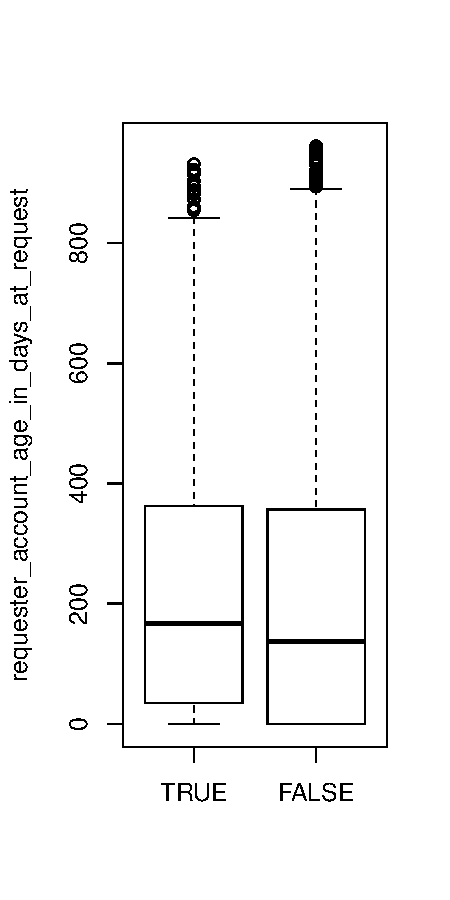
\includegraphics[width=0.16\textwidth]{data/requester_account_age_in_days_at_request}
	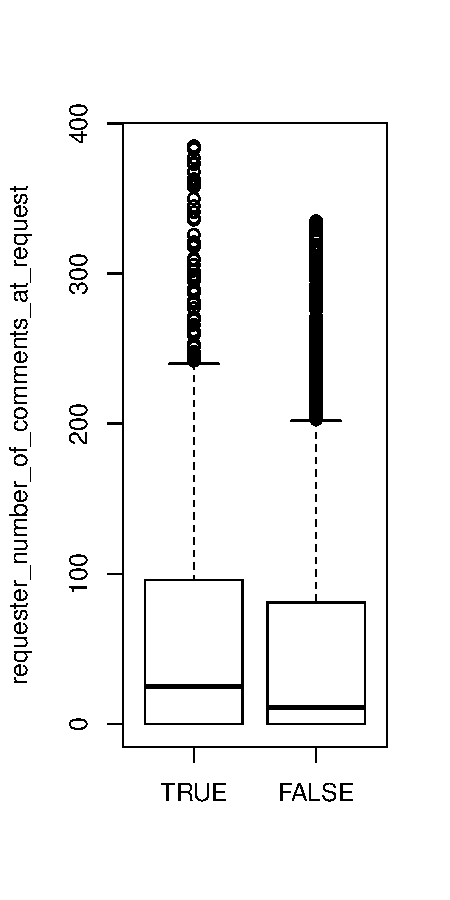
\includegraphics[width=0.16\textwidth]{data/requester_number_of_comments_at_request}
	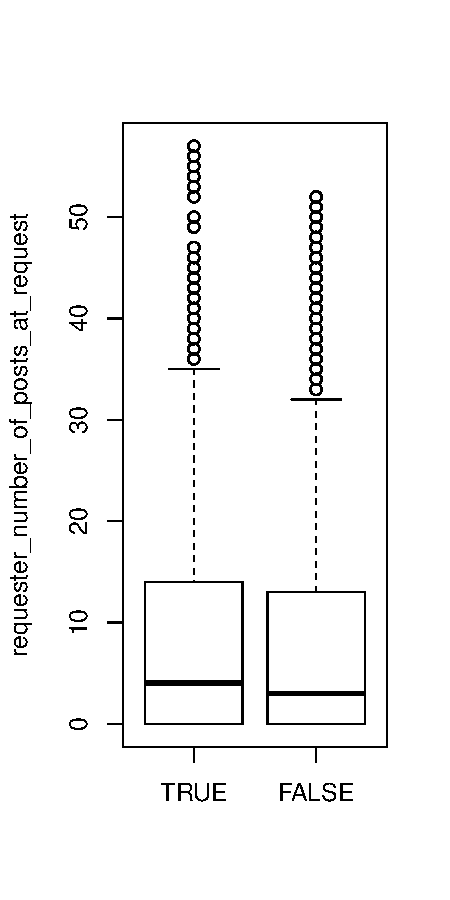
\includegraphics[width=0.16\textwidth]{data/requester_number_of_posts_at_request}
	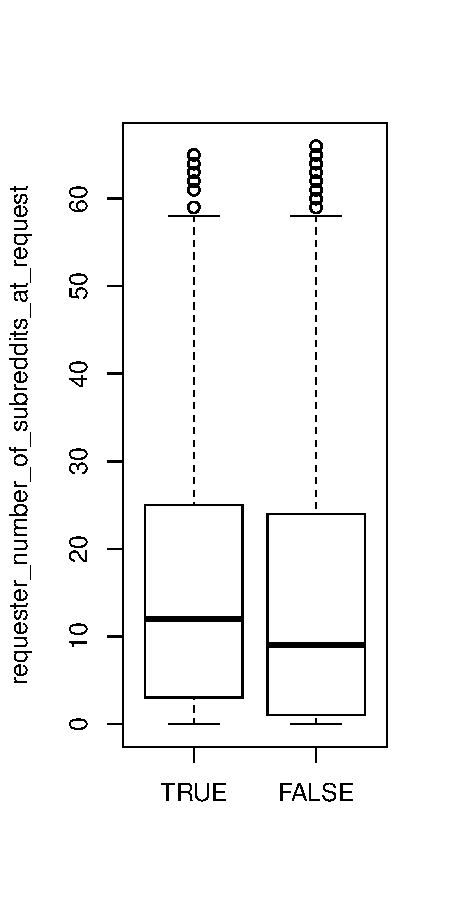
\includegraphics[width=0.16\textwidth]{data/requester_number_of_subreddits_at_request}
	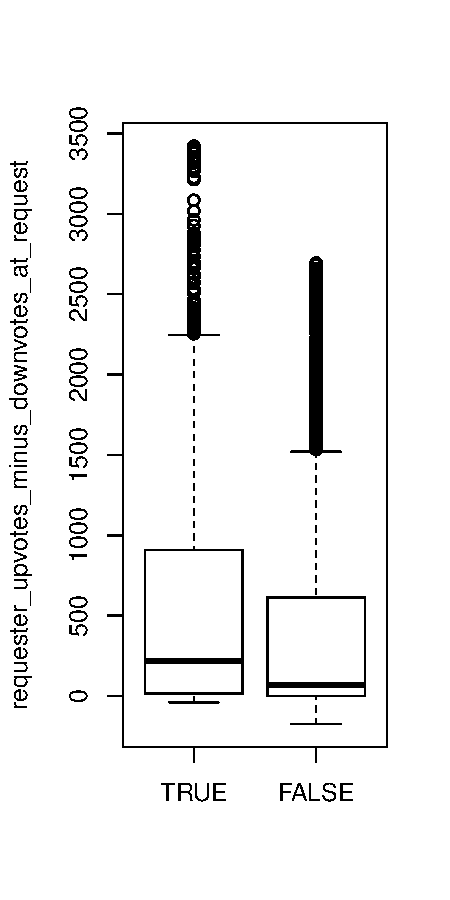
\includegraphics[width=0.16\textwidth]{data/requester_upvotes_minus_downvotes_at_request}
	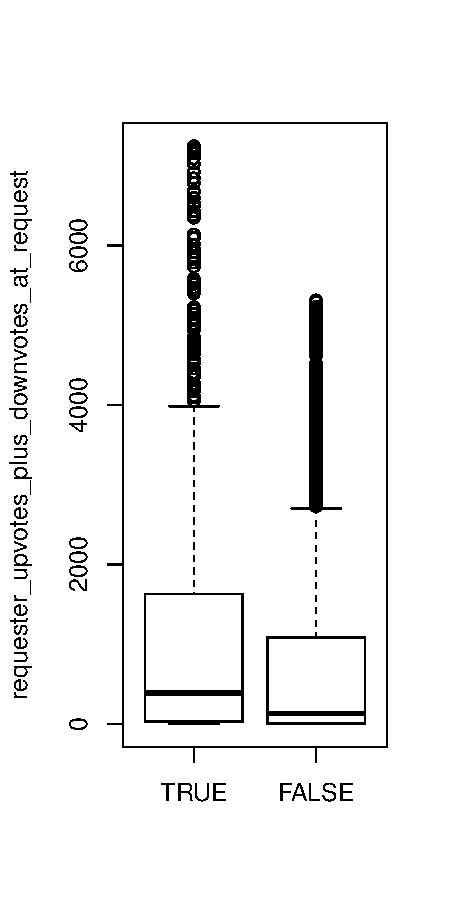
\includegraphics[width=0.16\textwidth]{data/requester_upvotes_plus_downvotes_at_request}
	\vspace*{-0.6cm}
	\caption{Boxplots of requester information attributes based on the success of requests}
	\vspace*{-0.6cm}
	\label{boxplot}
\end{figure}

\begin{table}[]
	\centering
	\caption{The confusion matrix for a fold in the cross validation}
	\label{confusion1}
	\begin{tabular}{|c|c|c|c|}
		\hline
		\multicolumn{2}{|c|}{\multirow{2}{*}{}}                & \multicolumn{2}{c|}{Actual}                            \\ \cline{3-4} 
		\multicolumn{2}{|c|}{}                                 & \multicolumn{1}{c|}{TRUE} & \multicolumn{1}{c|}{FALSE} \\ \hline
		\multicolumn{1}{|c|}{\multirow{2}{*}{Predict}} & TRUE  & 0                         & 0                          \\ \cline{2-4} 
		\multicolumn{1}{|c|}{}                         & FALSE & 92                        & 312                        \\ \hline
	\end{tabular}
	\vspace*{-0.6cm}
\end{table}

\subsection{Outcome prediction}
In second analysis, we perform a request classification task using requester information attributes to verify our assumption. There are several prediction models can be used in this classification task such as decision trees, logistic regression, SVM, etc. In our experiment, we used a simple logistic regression as the prediction method. We also used $10$-fold cross validation to measure the accuracy of the prediction model. At the iteration $i$ in the cross validation, we used fold $i$ as test set and the remaining data as training set. To measure the accuracy of the prediction model, we used the $F$-measure\footnote{\url{https://en.wikipedia.org/wiki/F1_score}}. The overall $F$-measure is 0. The reason why the value of the $F$-measure is zero is that the classifier always predict that a request will not receive a pizza. Table \ref{confusion1} show here a confusion matrix in a fold of the cross validation. We can see that the classifier predict \texttt{FALSE} values. From the experiment, we see that prediction models based requester information attributes do not perform well. It suggests that the decision whether or not a request receive a pizza do not based on the information about requester.

